% KAJIAN PUSTAKA 3

\begin{frame}
    \begin{columns}
        \begin{column}{0.35\textwidth}
            \LARGE
            Kajian Pustaka 3
        \end{column}
        \begin{column}{0.6\textwidth}
            \justifying
            \textbf{Judul:}\\
            A novel hybrid fusion algorithm for low-cost GPS/INS integrated navigation system during GPS outages

            \vspace{1.5em}

            \textbf{Penulis:}\\
            Li, Dengao; Jia, Xuan; Zhao, Jumin

            \vspace{1.5em}
            
            \textbf{Publikasi:}\\
            IEEE Access, vol.8, p.53984-53996, 2020
        \end{column}
    \end{columns}
\end{frame}


\begin{frame}
    \frametitle{Pustaka 3: Pendahuluan}
    \large
    \begin{itemize}
        \justifying
        \item Metode hybrid GPS / INS yang diusulkan dapat mendeteksi posisi dengan tepat walaupun terdapat GPS outage dan menggunakan GPS berbiaya rendah.
        \vspace{1em}
        \item Menggunakan Extreme Learning Machine untuk memberikan estimasi error INS terhadap GPS pada saat GPS padam.
        \vspace{1em}
        \item Pada saat GPS menyala, data error GPS digunakan untuk melakukan training ELM
    \end{itemize}
\end{frame}


\begin{frame}
    \frametitle{Pustaka 3: Skema Sistem}
    \centering
    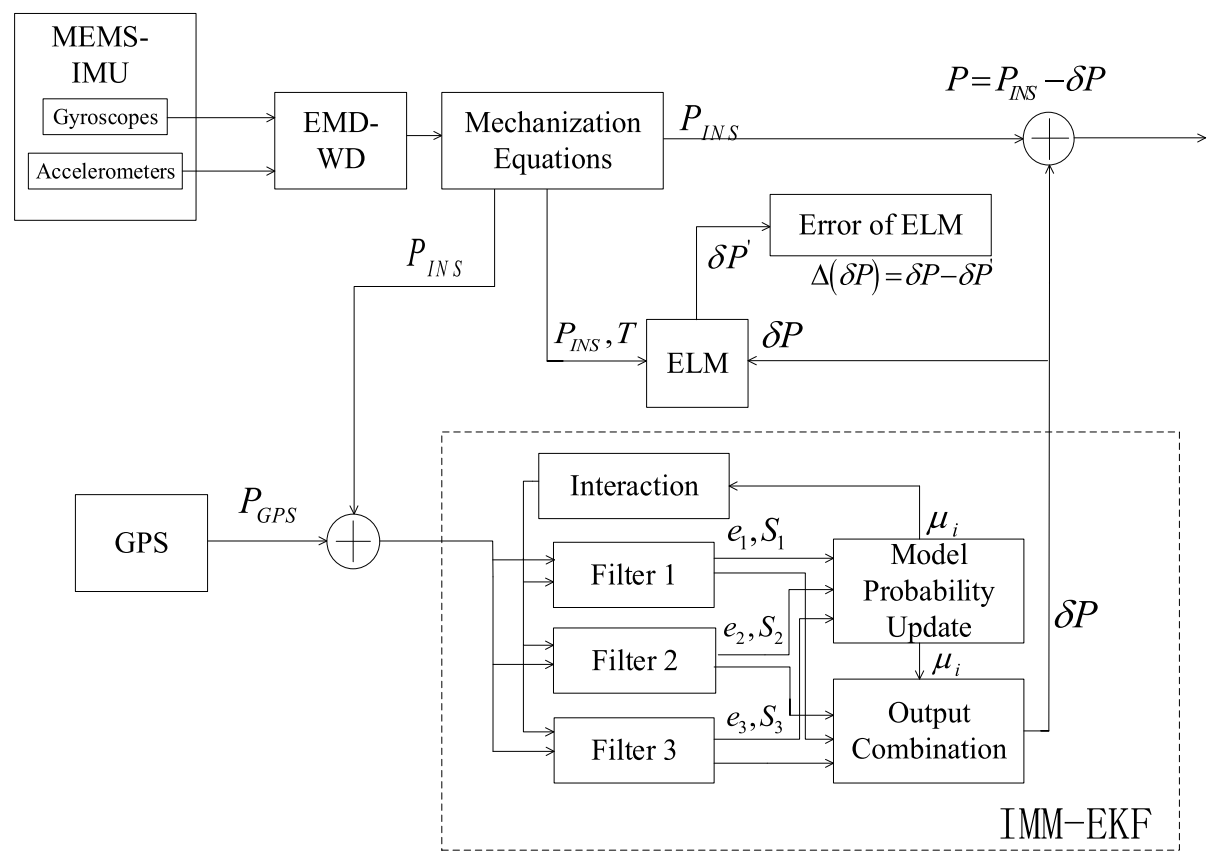
\includegraphics[width=.6\textwidth]{2-GPSINS-diagram.png}
\end{frame}


\begin{frame}[allowframebreaks]
    \frametitle{Pustaka 3: Metode. Bagian}
    \begin{enumerate}
        \justifying
        \item Hasil pembacaan INS difilter menggunakan Empirical Mode Decomposition Wavelet Denoising (EMD-WD).
        \vspace{1em}
        \item Hasil filter EMD-WD dimasukkan ke persamaan mekanisasi INS untuk mendapatkan posisi dan kecepatan.
        \vspace{1em}
        \item Posisi INS dan GPS dimasukkan ke Imterctive Multi-Model Kalman Filter (IMM-EKF) untuk mendapatkan error posisi untuk mengkoreksi INS.
        \vspace{1em}
        \pagebreak
        \item Apabila data GPS tersedia, Hasil persamaan mekanisasi INS, dan error posisi untuk koreksi INS yang dihasilkan IMM-EKF dijadikan sebagai data training untuk ELM.
        \vspace{1em}
        \item Apabila terjadi blackout, data keluaran IMM-EKF yang membutuhkan GPS diubah menjadi data keluaran ELM menggunakan masukkan dari persamaan mekanisasi INS.
    \end{enumerate}
\end{frame}


\begin{frame}
    \frametitle{Pustaka 3: Sistem saat blackout}
    \centering
    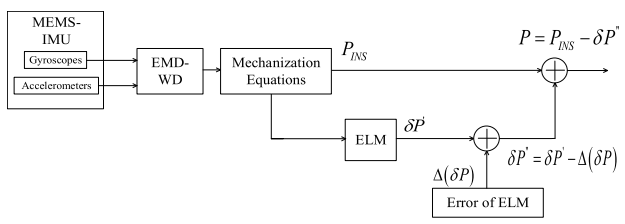
\includegraphics[width=.8\textwidth]{r3-prediksi.png}
\end{frame}


\begin{frame}
    \frametitle{Pustaka 3: EMD-WD}
    \centering
    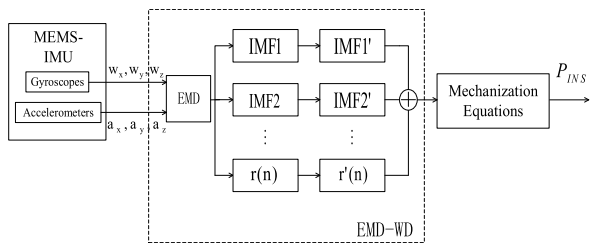
\includegraphics[width=.8\textwidth]{r3-EMDWD.png}
\end{frame}


\begin{frame}
    \frametitle{Pustaka 3: ELM}
    \centering
    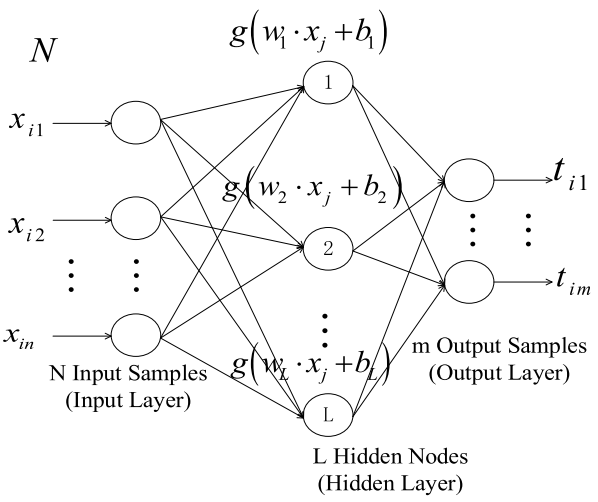
\includegraphics[width=.5\textwidth]{r3-ELM.png}
\end{frame}


\begin{frame}
    \frametitle{Pustaka 3: Hasil}
    \centering
    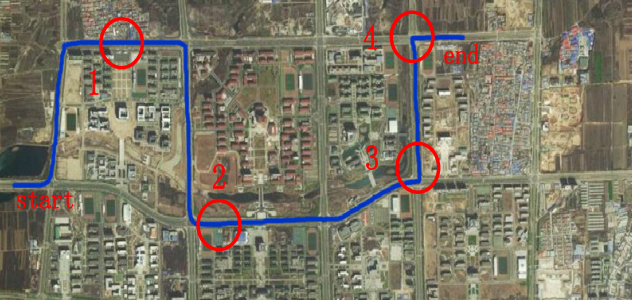
\includegraphics[width=.8\textwidth]{r3-hasil1.png}\\
    uji lapangan dengan lingkaran merah merupakan lokasi blackout GPS.
\end{frame}


\begin{frame}
    \frametitle{Pustaka 3: Hasil}
    \centering
    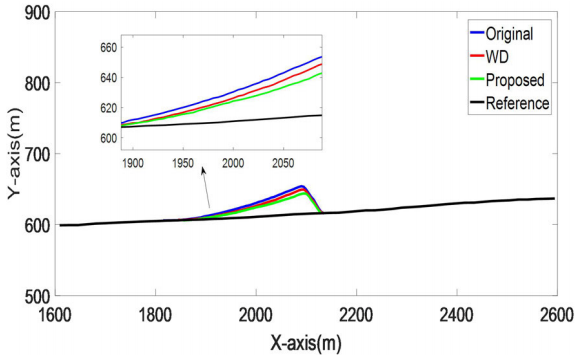
\includegraphics[width=.6\textwidth]{r3-hasil2.png}\\
    drift error pada wilayah uji 1
\end{frame}


\begin{frame}
    \frametitle{Pustaka 3: Kesimpulan}

    \large
    \textbf{Kelebihan}\\
    \normalsize
    \begin{itemize}
        \item Metode fusion hybrid INS dengan GPS pada penelitian ini dapat mengurangi drift error pada posisi INS saat tidak terdapat informasi dari GPS.
    \end{itemize}

    \large
    \textbf{Ide}\\
    \normalsize
    \begin{itemize}
        \item Algoritma fusi hybrid INS-GPS pada penelitian ini dapat digunakan sepenuhnya sebagai sub-sistem integrasi INS-GPS.
        \item posisi kendaraan yang dihasilkan oleh algoritma ini akan digunakan untuk mengubah posisi halangan yang dideteksi dari yang sebelumnya relatif terhadap kendaraan menjadi relatif terhadap bumi.
    \end{itemize}

\end{frame}
